\documentclass[aspectratio=169,14pt,usenames,dvipsnames]{beamer}
\usetheme{TalentSprint}
\usepackage[utf8]{inputenc}
\usepackage{graphics}
\usepackage{ragged2e}
\usepackage{amsfonts}
\usepackage{xcolor}
\usepackage{mathtools}
\usepackage{tcolorbox}
\usepackage{setspace}
\usepackage{lmodern}
\definecolor{swe}{rgb}{0.19, 0.73, 0.56}
\definecolor{lgreen}{RGB}{190,200,198}
\title[KNN]{KNN}

\begin{document}

{\1
\begin{frame} \vspace{35pt}
%	\title[KNN]{KNN}
	\subtitle{Classification Algorithms}
	\maketitle
\end{frame}
}


\begin{frame}{Formalized Folk Wisdom $\Rightarrow$  kNN}
\begin{itemize}
\item “Ornithological species of identical plumage congregate concurrently”
\item Argument by analogy
\item Classify an unknown sample by looking at its “neighbors”
\end{itemize}
\end{frame}

\begin{frame}{Goal: Classify Unknown Samples}
\begin{itemize}
\item Two features
\setbeamertemplate{itemize, items}[circle]
\begin{itemize}
\item Only for plotting convenience
\end{itemize}
\item Training: 10 RED + 10 GREEN
\item Testing: 5 BLACK
\end{itemize}
\end{frame}

\begin{frame}{Graphical View}
\centering
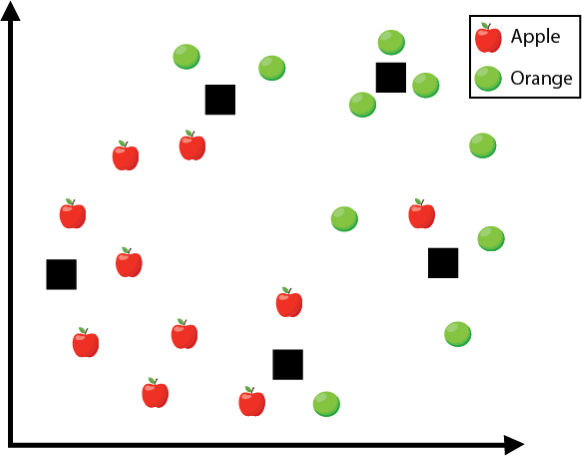
\includegraphics[width=6cm, height=5cm]{Images/4knn.png}
\end{frame}

\begin{frame}{But We Know!}
\centering
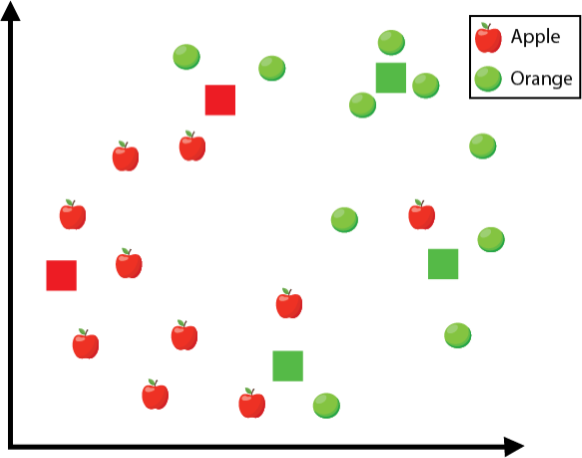
\includegraphics[width=6cm, height=5cm]{Images/5knn.png}
\end{frame}

\begin{frame}{First Look at kNN}
\begin{columns}
\column{0.5\textwidth}
\alert{Recall the idea:}
\begin{itemize}
  \item Group by ``nearness"
\end{itemize}
\alert{Method:}
\begin{itemize}
\item Determine 3 nearest neighbors
\item Assign majority label
\end{itemize}
\column {0.5\textwidth}
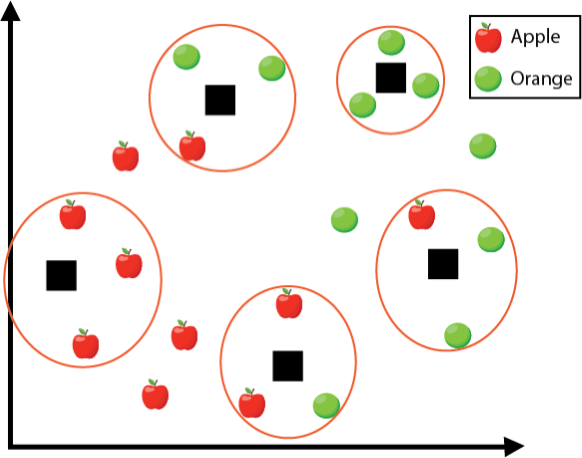
\includegraphics[width=0.8\textwidth, height=0.6\textheight]{Images/6knn.png}
\end{columns}
\end{frame}


\begin{frame}{What is the Accuracy?}
\begin{itemize}
\item 3 out of 5 got correct:
\setbeamertemplate{itemize, items}[circle]
\begin{itemize}
\item Accuracy = 60\%
\item Error = 40\%
\end{itemize}
\item Is it good or bad or ugly?
\item<2> A random guess could have given 50\%!!
\end{itemize}
\end{frame}


\begin{frame}{Comments}
\begin{itemize}
\item We “assumed” k = 3. It can also be 5, 7 … 10 
\setbeamertemplate{itemize, items}[circle]
\begin{itemize}
\item often odd. Why?
\end{itemize}
\item The data can have many more classes
\setbeamertemplate{itemize, items}[circle]
\begin{itemize}
\item Apples, Oranges and Mangoes
\end{itemize}
\item Distances need not be Euclidean. 
\setbeamertemplate{itemize, items}[circle]
\begin{itemize}
\item Other distance functions exist
\end{itemize}
\end{itemize}
\end{frame}


\begin{frame}{Will Another k Help? Some Times.}
\begin{columns}
\column{0.5\textwidth}
\alert{Idea:}
\begin{itemize}
  \item Try and pick the best
\end{itemize}
\alert{Method:}
\begin{itemize}
\item Try k = 5
\item What is the Accuracy?
\setbeamertemplate{itemize, items}[circle]
\begin{itemize}
\item<2> 80\%
\end{itemize}
\end{itemize}
\column {0.5\textwidth}
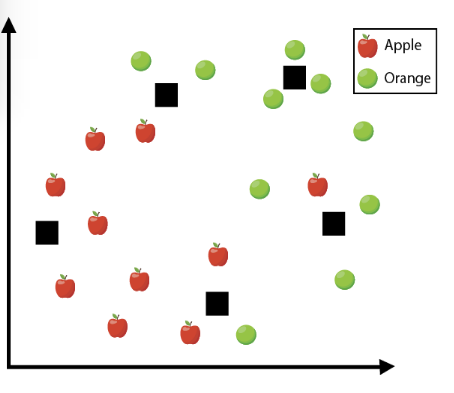
\includegraphics[width=7cm, height=6cm]{Images/9knn.png}
\end{columns}
\end{frame}

\begin{frame}{k Nearest Neighbours (kNN)}
\begin{tcolorbox}[width=13cm,left=0pt,boxrule=0.2pt,sharp corners, right=0pt,colback={lgreen!60!white}]
\textbf{\textcolor{red}{Given k, Data and Distance Function}}
\begin{itemize}
\item Find the distance from z to all the samples in X
\item Identify the k-Nearest Neighbours (smallest distances) and their class          labels
\item Classify z as the majority label from the k-Nearest Neighbours
\end{itemize}
\end{tcolorbox}
\end{frame}
	
\begin{frame}{Characteristics}
\begin{itemize}
\item KNN: n distance computations each of O(d) \\
\begin{itemize} \item number of samples = n
		\item  number of features or dimensionality = d
\end{itemize}
\item Too many operations
\item Needs all training samples at test time
\item Storage intensive
\item Computation intensive
\end{itemize}
\end{frame}


\begin{frame}{Outlier}
\begin{itemize}
\item If a sample is not in the “K Neighbours ” of at least one sample, it is an outlier \\
\centering
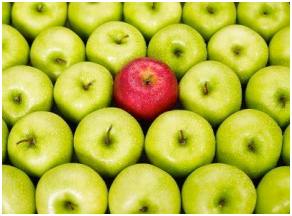
\includegraphics[width=4.5cm , height=3.5cm]{Images/12knn.png}
\end{itemize}
\end{frame}


\begin{frame}{Epsilon Neighbourhood}
\begin{itemize}
\item Samples within a radius of $\epsilon$  from  an sample \\
\centering
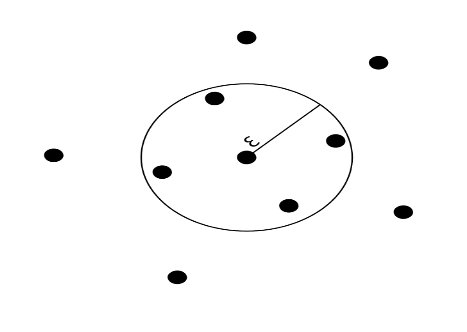
\includegraphics[width=6cm , height=6cm]{Images/knn13.png}
\end{itemize}
\end{frame}


\begin{frame}{Experiment}
\begin{itemize}
\item {Demo\_KNN\_Scaling}
	\begin{itemize}
		\item Dataset : Fruits 
		\item Objective : How characteristics of the data affect KNN effectiveness 
	\end{itemize}
\end{itemize}
\end{frame}

{\1
\begin{frame}
	\title{Scaling}
\titlepage
\end{frame}
}

\begin{frame}[t]{How Scaling Affects the kNN?}
\begin{figure}
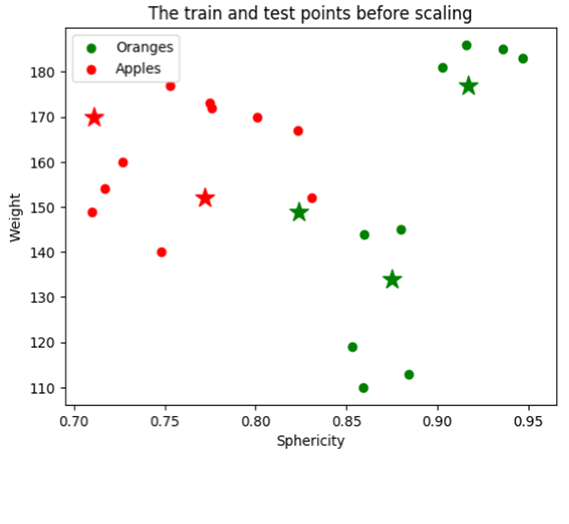
\includegraphics[width=6cm, height=5cm]{Images/13knn.png}
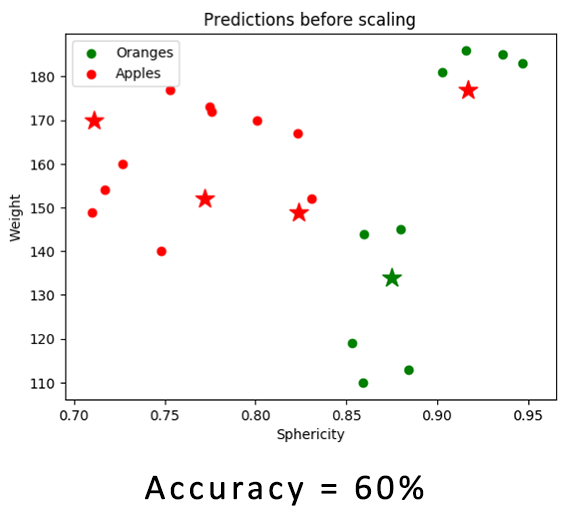
\includegraphics[width=6cm, height=5cm]{Images/14knn.png}
\end{figure}
\end{frame}


\begin{frame}[t]{How Scaling Affects the kNN?}
\begin{columns}
\column{0.5\textwidth}
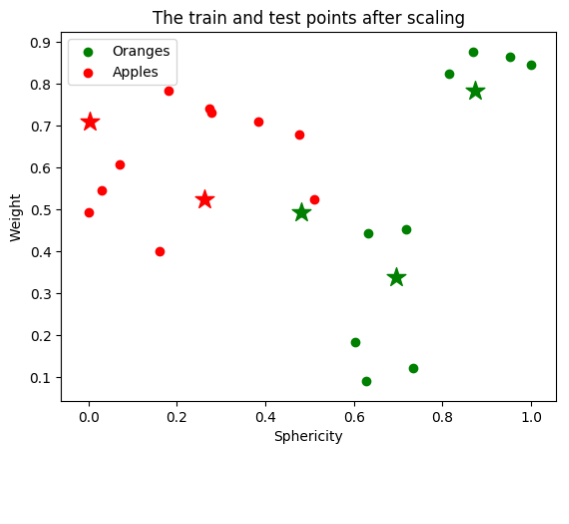
\includegraphics[width=6cm, height=4cm]{Images/13aknn.png}
\column{0.5\textwidth}
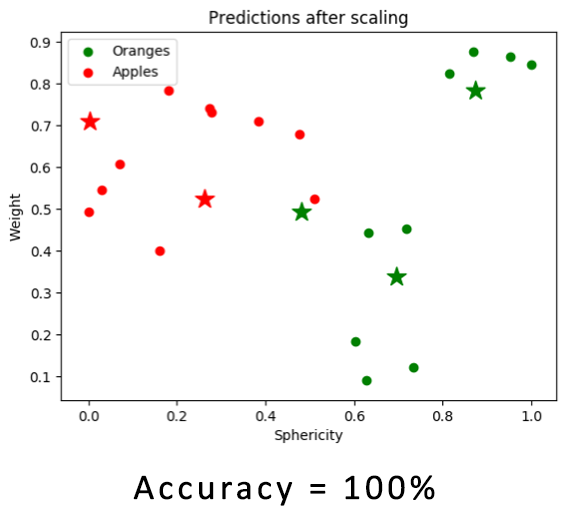
\includegraphics[width=6cm, height=4cm]{Images/14aknn.png}
\end{columns}

\vspace{0.5cm}\centering
\small {There is a change in the accuracy before and  after scaling the data.}
\end{frame}

\begin{frame}{Distance Functions}
\begin{itemize}
\item Used to measure similarity between samples
\item Different types in different contexts
\item Examples:
	\begin{itemize}
		\item Euclidean 
		\item Manhattan 
		\item Minkowski 
		\item Hamming
	\end{itemize}
\end{itemize}
\end{frame}

\begin{frame}{Distance Functions}
\centering
\begin{itemize}
	\item \small{Euclidean $$\sqrt{\sum_{i=1}^k{(x_i - x'_i)^2}}$$ } \\[2pt]
	\item \small{Manhattan $$\sum_{i=1}^k{|x_i - x'_i|}$$}
\end{itemize}
\end{frame}

\begin{frame}{Distance Functions}
\vspace{0.5cm}\centering
\begin{itemize}
	\item \small{Minkowski:      $$ \Bigg(    \sum_{i=1}^k{({|x_i - x'_i|})^q}  \Bigg)^{1/q} $$} \\[5pt]
	\item \small{Hamming:         $$D_H = \sum_{i=1}^k{|x_i - x'_i|} $$}
%\vspace{0.1cm}
\end{itemize}	\vspace{0.13cm}     \small{\hspace{1.5cm}$ \alert{ x = x' \Rightarrow D = 0} $}\\ \small{\hspace{1.5cm}$ \alert{x \neq x' \Rightarrow D = 1} $}

%\end{itemize}
\end{frame}


\begin{frame}{Experiments : }
\begin{itemize}
\item {Demo\_KNN\_Advertising\_data} 
	\begin{itemize}
		\item Dataset : Advertising  
		\item Objective : To classify the data using KNN classifier
	\end{itemize}

\end{itemize}
\end{frame}


{ \1
\begin{frame}
	\title{Thanks!!}
	\subtitle{Questions?}
	\maketitle
\end{frame}
}

\end{document}
